%! Author = Profesor
%! Date = 06/06/2024


\section{Ejercicios PAU}

\begin{exerciseEVAU}
    Complete las siguientes reacciones orgánicas:
    \begin{enumerate}[label=\letraminuscula]
        \item \ch{CH2=CH2 + HBr ->}
        \item \ch{CH3CH2CH2OH + H2SO4 ->}
        \item \ch{C4H10 + O2 ->}
        \item \ch{CH3CH2CH2COOH + CH3CH2CH2OH ->}
    \end{enumerate}
\begin{solu}
    
\end{solu}
\end{exerciseEVAU}

\begin{exerciseEVAU}
    De los siguientes pares de compuestos, ¿cuáles son isómeros? ¿Qué tipo de
    isomería presentan?
    \begin{enumerate}[label=\letraminuscula]
        \item
        \begin{figure}[H]
            \centering
            % [FIGURA ORIGINAL] \includegraphics{images/imagesUD9Organica/UD9_Problemas/T9_EvAU_02_a}
            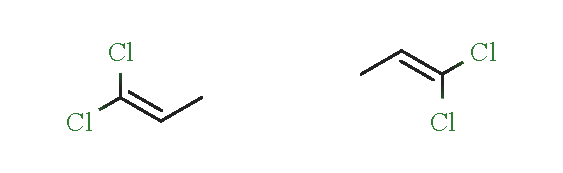
\includegraphics[width=0.45\linewidth]{FigurasSVG/UD9_Quimica_Organica/pdf/UD9_E01_dicloropropeno.pdf}
        \end{figure}
        \item
        \begin{figure}[H]
            \centering
            % [FIGURA ORIGINAL] \includegraphics{images/imagesUD9Organica/UD9_Problemas/T9_EvAU_02_b}
            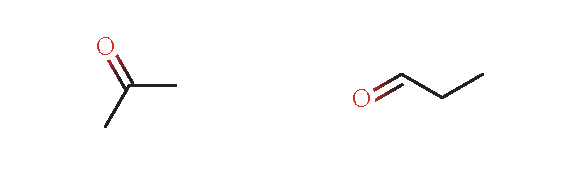
\includegraphics[width=0.45\linewidth]{FigurasSVG/UD9_Quimica_Organica/pdf/UD9_E02_propanona_propanal.pdf}
        \end{figure}
        \item
        \begin{figure}[H]
            \centering
            % [FIGURA ORIGINAL] \includegraphics{images/imagesUD9Organica/UD9_Problemas/T9_EvAU_02_C}
            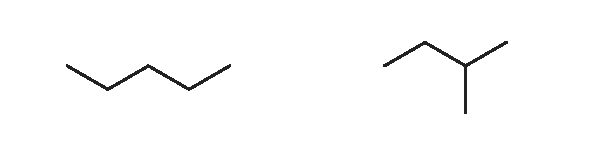
\includegraphics[width=0.47\linewidth]{FigurasSVG/UD9_Quimica_Organica/pdf/UD9_E03_pentano_metilbutano.pdf}
        \end{figure}
        \item
        \begin{figure}[H]
            \centering
            % [FIGURA ORIGINAL] \includegraphics{images/imagesUD9Organica/UD9_Problemas/T9_EvAU_02_D}
            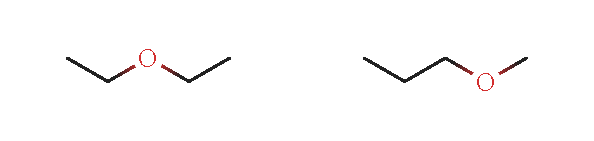
\includegraphics[width=0.47\linewidth]{FigurasSVG/UD9_Quimica_Organica/pdf/UD9_E04_eteres.pdf}
        \end{figure}
    \end{enumerate}

    \begin{solu}
        \begin{enumerate}[label=\letraminuscula]
            \item Ambas estructuras representan la molécula \ch{CH3-CH=CCl2} (1,1-dicloroprop-1-eno), dibujada de dos formas distintas (intercambiando las posiciones del \ch{H} y del \ch{CH3} sobre el carbono no clorado). Como el otro carbono del doble enlace lleva \textbf{dos sustituyentes iguales} (\ch{Cl} y \ch{Cl}), no existe posibilidad de isomería geométrica cis-trans en esta molécula: ambos dibujos son la \textbf{misma sustancia}, no son isómeros.

            \item La primera estructura es la propanona (acetona), \ch{CH3-CO-CH3}, y la segunda es el propanal, \ch{CH3-CH2-CHO}. Ambas tienen la misma fórmula molecular \ch{C3H6O} pero distinto grupo funcional (cetona frente a aldehído), por lo que son \textbf{isómeros de función}.

            \item La primera estructura es el pentano, \ch{CH3-CH2-CH2-CH2-CH3}, y la segunda es el 2-metilbutano, \ch{CH3-CH(CH3)-CH2-CH3}. Ambas responden a la fórmula molecular \ch{C5H12}: la primera es una cadena lineal y la segunda ramificada, por lo que son \textbf{isómeros de cadena}.

            \item La primera estructura es el dietil éter (etoxietano), \ch{CH3-CH2-O-CH2-CH3}, y la segunda es el metil propil éter (1-metoxipropano), \ch{CH3-O-CH2-CH2-CH3}. Ambas tienen fórmula molecular \ch{C4H10O} y el mismo grupo funcional (éter), pero el oxígeno ocupa una posición distinta de la cadena carbonada, por lo que son \textbf{isómeros de posición}.
        \end{enumerate}
    \end{solu}
\end{exerciseEVAU}

\begin{exerciseEVAU}
    Indique el nombre de cada grupo funcional en las siguientes moléculas.

    \begin{enumerate}[label=\letraminuscula]

    \item
    \begin{figure}[H]
        \centering
        % [FIGURA ORIGINAL] \includegraphics{images/imagesUD9Organica/UD9_Problemas/T9_EvAU_03_a}
        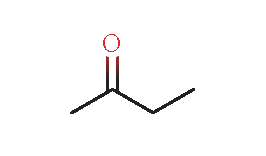
\includegraphics[width=0.21\linewidth]{FigurasSVG/UD9_Quimica_Organica/pdf/UD9_E05_butanona.pdf}
    \end{figure}
    \begin{figure}[H]
        \centering
        % [FIGURA ORIGINAL] \includegraphics{images/imagesUD9Organica/UD9_Problemas/T9_EvAU_03_b}
        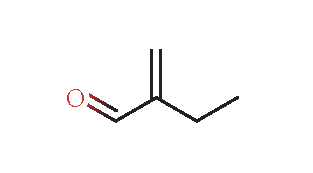
\includegraphics[width=0.25\linewidth]{FigurasSVG/UD9_Quimica_Organica/pdf/UD9_E06_aldehido_insaturado.pdf}
    \end{figure}

    \item \ch{HOOC-CH2-CH2-CHNH-CH3}

    \item
    \begin{figure}[H]
        \centering
        % [FIGURA ORIGINAL] \includegraphics{images/imagesUD9Organica/UD9_Problemas/T9_EvAU_03_d}
        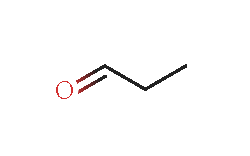
\includegraphics[width=0.20\linewidth]{FigurasSVG/UD9_Quimica_Organica/pdf/UD9_E07_propanal.pdf}
    \end{figure}
    \end{enumerate}
    \begin{solu}
        \begin{enumerate}[label=\letraminuscula]
            \item La primera estructura es el \ch{CH3-CH2-CO-CH3} (butan-2-ona): el grupo carbonilo está unido a dos átomos de carbono, por lo que se trata de una \textbf{cetona}. La segunda estructura representa una cadena carbonada con un grupo \ch{-CHO} terminal (\textbf{aldehído}) combinada con un doble enlace \ch{C=C} (\textbf{alqueno}); es decir, un \textbf{aldehído insaturado}.

            \item \(\ch{HOOC-CH2-CH2-CH(NH2)-CH3}\): la molécula presenta dos grupos funcionales: un grupo \ch{-COOH} (\textbf{ácido carboxílico}) en un extremo de la cadena y un grupo \ch{-NH2} (\textbf{amina primaria}) sobre el carbono próximo al otro extremo.

            \item La estructura es \ch{CH3-CH2-CHO} (propanal): el grupo carbonilo está unido a un átomo de H y a un átomo de C, por lo que se trata de un \textbf{aldehído}.
        \end{enumerate}
    \end{solu}
\end{exerciseEVAU}

\begin{exerciseEVAU}
    \begin{enumerate}[label=\letraminuscula]
        \item En los siguientes compuestos, indique qué tipo de hibridación presenta cada carbono:

        \ch{CH3-COOH}  y  \ch{CH3-C~C-CH3}
        \item De los siguientes compuestos, diga si son ópticamente activos y razone su respuesta.

        \ch{CH2OH-CHBr-COOH} Y \ch{CH3CH2-COOH}
    \end{enumerate}

    \begin{solu}
        \begin{enumerate}[label=\letraminuscula]
            \item En \ch{CH3-COOH} (ácido etanoico): el carbono del grupo \ch{CH3} está unido únicamente por enlaces sencillos (a 3 \ch{H} y al otro carbono), por lo que presenta hibridación \(sp^3\); el carbono del grupo \ch{-COOH} forma un doble enlace con el oxígeno (\ch{C=O}) y enlaces sencillos con \ch{-OH} y con \ch{-CH3}, por lo que presenta hibridación \(sp^2\).

            En \ch{CH3-C~C-CH3} (but-2-ino): los dos carbonos de los grupos \ch{CH3} (extremos) tienen hibridación \(sp^3\); los dos carbonos unidos por el triple enlace \ch{C~C} tienen hibridación \(sp\) (cada uno forma un enlace \(\sigma\) con un grupo metilo, un enlace \(\sigma\) con el otro carbono del triple enlace y dos enlaces \(\pi\) perpendiculares entre sí).

            \item \ch{CH2OH-CHBr-COOH} (ácido 3-hidroxi-2-bromopropanoico): el carbono central (\ch{CHBr}) está unido a cuatro sustituyentes distintos: \ch{-CH2OH}, \ch{-Br}, \ch{-COOH} y \ch{-H}. Al tener cuatro grupos diferentes se trata de un \textbf{carbono asimétrico o quiral}, por lo que la molécula es \textbf{ópticamente activa} (presenta dos enantiómeros).

            \ch{CH3-CH2-COOH} (ácido propanoico) no posee ningún carbono unido a cuatro sustituyentes distintos (el \ch{C2} tiene dos \ch{H} iguales), por lo que \textbf{no es ópticamente activo}.
        \end{enumerate}
    \end{solu}
\end{exerciseEVAU}

\begin{exerciseEVAU}
    \begin{enumerate}[label=\letraminuscula]
        \item
        \begin{enumerate}[label=\letraminuscula]
            \item  Dibuje los isómeros geométricos de la molécula

            \ch{CH3-CH2-CH2-CH=CH-CH2-CH2-CH3}

            \item  Dibuje los isómeros geométricos de la molécula

            \ch{CH3-CH2-CH2-COOH}
        \end{enumerate}
        \item
        \begin{enumerate}[label=\letraminuscula]
            \item Escriba un isómero de fórmula molecular C4H10O que presente actividad óptica Escriba un isómero de fórmula molecular \ch{C4H10O} que presente actividad óptica.
            \item
            \item Escriba dos isómeros correspondientes a la fórmula molecular \ch{5H12}
        \end{enumerate}
    \end{enumerate}

    \begin{solu}
        \begin{enumerate}[label=\letraminuscula]
            \item
            \begin{enumerate}[label=\letraminuscula]
                \item El oct-4-eno, \ch{CH3-CH2-CH2-CH=CH-CH2-CH2-CH3}, presenta isomería geométrica porque cada carbono del doble enlace lleva dos sustituyentes distintos (\ch{H} y \ch{CH2-CH2-CH3}):
                \begin{itemize}
                    \item \emph{cis}-oct-4-eno: los dos grupos propilo (\ch{-CH2CH2CH3}) quedan al mismo lado del doble enlace.
                    \item \emph{trans}-oct-4-eno: los dos grupos propilo quedan en lados opuestos del doble enlace.
                \end{itemize}

                \item \ch{CH3-CH2-CH2-COOH} (ácido butanoico) no presenta isomería geométrica, ya que no contiene ningún doble enlace \ch{C=C}: el único doble enlace de la molécula es el \ch{C=O} del grupo carboxilo, que no puede dar lugar a isomería cis-trans.
            \end{enumerate}

            \item
            \begin{enumerate}[label=\letraminuscula]
                \item Butan-2-ol, \ch{CH3-CH(OH)-CH2-CH3}, presenta actividad óptica: el carbono 2 está unido a cuatro sustituyentes distintos (\ch{-OH}, \ch{-CH3}, \ch{-CH2CH3} y \ch{-H}), por lo que es un carbono asimétrico.

                \item Para la fórmula molecular \ch{C5H12} (pentanos), dos isómeros posibles son:
                \begin{itemize}
                    \item Pentano: \ch{CH3-CH2-CH2-CH2-CH3}
                    \item 2-metilbutano: \ch{CH3-CH(CH3)-CH2-CH3}
                \end{itemize}
                (también sería válido el 2,2-dimetilpropano, \ch{C(CH3)4}).
            \end{enumerate}
        \end{enumerate}
    \end{solu}
\end{exerciseEVAU}

\begin{exerciseEVAU}
    \begin{enumerate}[label=\letraminuscula]
        \item Dibuje los isómeros geométricos cis-trans de 3-hexeno.
        \item Escriba todos los isómeros de fórmula molecular \ch{C5H12}.
        \item Escriba el producto resultante de las siguientes reacciones orgánicas:
        \begin{itemize}
            \item \ch{CH3-CH=CH-CH3 + HCl -> }
            \item \ch{CH3-CH2-CH2-CH2-OH + H2SO4 ->}
        \end{itemize}

    \end{enumerate}
    \begin{solu}
        \begin{enumerate}[label=\letraminuscula]
            \item El 3-hexeno, \ch{CH3-CH2-CH=CH-CH2-CH3}, tiene en cada carbono del doble enlace un \ch{H} y un grupo etilo (\ch{-CH2CH3}), sustituyentes distintos, por lo que presenta isomería cis-trans:
            \begin{itemize}
                \item \emph{cis}-3-hexeno: los dos grupos etilo al mismo lado del doble enlace.
                \item \emph{trans}-3-hexeno: los dos grupos etilo en lados opuestos.
            \end{itemize}

            \item Los isómeros de fórmula molecular \ch{C5H12} son tres:
            \begin{itemize}
                \item Pentano: \ch{CH3-CH2-CH2-CH2-CH3}
                \item 2-metilbutano (isopentano): \ch{CH3-CH(CH3)-CH2-CH3}
                \item 2,2-dimetilpropano (neopentano): \ch{C(CH3)4}
            \end{itemize}

            \item
            \begin{itemize}
                \item \ch{CH3-CH=CH-CH3 + HCl -> CH3-CH2-CHCl-CH3}. Es una reacción de adición electrófila de un hidrácido a un alqueno simétrico (but-2-eno); al ser los dos carbonos del doble enlace equivalentes, se obtiene un único producto: 2-clorobutano.

                \item \ch{CH3-CH2-CH2-CH2-OH + H2SO4 ->[Calor] CH3-CH2-CH=CH2 + H2O}. Es una reacción de eliminación (deshidratación intramolecular) del butan-1-ol catalizada por ácido sulfúrico concentrado en caliente, que da lugar al but-1-eno (y agua).
            \end{itemize}
        \end{enumerate}
    \end{solu}
\end{exerciseEVAU}


\begin{exerciseEVAU}
    Indique que tipo de reacción orgánica tiene lugar en cada uno de los siguientes procesos.
    \begin{enumerate}[label=\letraminuscula]
        \item \ch{CH3-CH2-CHO -> CH3-CH2-CH2-OH}
        \item \ch{CH3-CH2-CH2-OH -> CH3-CH=CH2}
        \item \ch{CH3-CH=CH2 - CH3-CH2-CH2-Br }
        \item \ch{CH3-CH2-COOH + CH3-CH2-CH2-OH -> CH3-CH2-COO-CH2-CH2-CH3 }
        \item \ch{CH3-CH2-CH2-OH -> CH3-CH3-CHO}
    \end{enumerate}
    \begin{solu}
        \begin{enumerate}[label=\letraminuscula]
            \item \textbf{Reducción} del propanal (\ch{CH3-CH2-CHO}) a propan-1-ol (\ch{CH3-CH2-CH2-OH}) por adición de hidrógeno al grupo carbonilo.

            \item \textbf{Eliminación} (deshidratación) del propan-1-ol para dar propeno (\ch{CH3-CH=CH2}), con pérdida de una molécula de agua.

            \item \textbf{Adición} electrófila de \ch{HBr} al propeno, que sigue la regla de Markovnikov y da 1-bromopropano como producto mayoritario (\ch{CH3-CH2-CH2-Br}).

            \item \textbf{Sustitución} (esterificación): el ácido propanoico reacciona con el propan-1-ol para dar el propanoato de propilo y agua, catalizada por medio ácido.

            \item \textbf{Oxidación} del propan-1-ol (alcohol primario) a propanal, \ch{CH3-CH2-CHO} (la fórmula del producto en el enunciado contiene una errata, pues debería ser \ch{CH3-CH2-CHO} y no \ch{CH3-CH3-CHO}).
        \end{enumerate}
    \end{solu}
\end{exerciseEVAU}


\begin{exerciseEVAU}
    \textbf{2024}.
    \begin{enumerate}[label=\letraminuscula]
         \item Escriba las fórmulas de un isómero de cadena y otro de posición del siguiente compuesto:

         \ch{CH3–CH=CH–CH2–CH3}.

         \item \item Escriba la fórmula de un isómero de función de la butanona: \ch{CH3–CH2–CO–CH3}

    \end{enumerate}

    \begin{solu}
        \begin{enumerate}[label=\letraminuscula]
            \item El compuesto \ch{CH3-CH=CH-CH2-CH3} es el pent-2-eno (\ch{C5H10}).
            \begin{itemize}
                \item Isómero de \textbf{cadena} (mismo grupo funcional alqueno, distinta ramificación del esqueleto carbonado): 2-metilbut-2-eno, \ch{CH3-C(CH3)=CH-CH3}.
                \item Isómero de \textbf{posición} (mismo esqueleto lineal y mismo grupo funcional, doble enlace en otra posición): pent-1-eno, \ch{CH2=CH-CH2-CH2-CH3}.
            \end{itemize}

            \item La butanona, \ch{CH3-CH2-CO-CH3} (\ch{C4H8O}), es una cetona. Un isómero de función (mismo \ch{C4H8O}, distinto grupo funcional) es el aldehído butanal: \ch{CH3-CH2-CH2-CHO}.
        \end{enumerate}
    \end{solu}
\end{exerciseEVAU}

\begin{exerciseEVAU}
    \begin{enumerate}[label=\letraminuscula]
        \item Escriba las fórmulas de un isómero de cadena y otro de posición del siguiente compuesto:

        \ch{CH3-CH=CH-CH2-CH3}
        \item Escriba la fórmula de un isómero de función de la butanona:
        
        \ch{CH3-CH2-CO-CH3}
    \end{enumerate}
    \begin{solu}

    \end{solu}
\end{exerciseEVAU}

\begin{exerciseEVAU}
    \textbf{2023}. Complete las siguientes reacciones orgánicas:
    \begin{enumerate}[label=\letraminuscula]
    \item \ch{CH3CH2COOH + CH3CH2OH ->}
    \item \ch{CH2=CH2 + Br2 -> }
    \item \ch{C4H10 + O2 -> }
    \item \ch{CH2=CH2 + H2O ->[\( H2SO4 \)]}
    \end{enumerate}
    \begin{solu}
        \begin{enumerate}[label=\letraminuscula]
            \item \ch{CH3-CH2-COOH + CH3-CH2-OH ->[H+] CH3-CH2-COO-CH2-CH3 + H2O}. Es una \textbf{esterificación} (reacción de sustitución) entre el ácido propanoico y el etanol; se obtiene propanoato de etilo y agua.

            \item \ch{CH2=CH2 + Br2 -> CH2Br-CH2Br}. Es una \textbf{adición electrófila} de dibromo al eteno, que da 1,2-dibromoetano.

            \item \ch{C4H10 + 13/2 O2 -> 4CO2 + 5H2O}. Es una reacción de \textbf{combustión} (oxidación total) del butano.

            \item \ch{CH2=CH2 + H2O ->[H2SO4] CH3-CH2-OH}. Es una \textbf{adición electrófila} (hidratación catalizada por ácido) del eteno, que da etanol.
        \end{enumerate}
    \end{solu}
\end{exerciseEVAU}


\begin{exerciseEVAU}
    Escriba la reacción y nombre los productos obtenidos al someter al 1-butanol (butan-1-ol) a un proceso de:

    \begin{enumerate}[label=\letraminuscula]
        \item Combustión.
        \item Un posible producto de oxidación.
        \item Deshidratación.
        \item Reacción con ácido etanoico.
    \end{enumerate}

    \begin{solu}

%        \begin{figure}[H]
%            \centering
%            \includegraphics[scale=.6]{images/imagesUD9Organica/UD9_Problemas/Organica_EvAU_01.png}
%            %\caption{}
%            %\label{fig:}
%        \end{figure}

        \begin{enumerate}[label=\letraminuscula]
            \item Combustión: \ch{CH3-CH2-CH2-CH2-OH + 6O2 -> 4CO2 + 5H2O}. Reacción de oxidación total, muy exotérmica.

            \item Oxidación (suave, con un oxidante como el dicromato): al ser un alcohol primario se oxida primero a aldehído y, si el oxidante es fuerte, a ácido carboxílico. \ch{CH3-CH2-CH2-CH2-OH ->[ [O] ] CH3-CH2-CH2-CHO} (butanal) \ch{->[ [O] ] CH3-CH2-CH2-COOH} (ácido butanoico).

            \item Deshidratación (eliminación intramolecular, medio ácido y calor): \ch{CH3-CH2-CH2-CH2-OH ->[H2SO4, calor] CH3-CH2-CH=CH2 + H2O}, obteniéndose but-1-eno.

            \item Reacción con ácido etanoico (esterificación): \ch{CH3-CH2-CH2-CH2-OH + CH3-COOH ->[H+] CH3-COO-CH2-CH2-CH2-CH3 + H2O}, obteniéndose el etanoato de butilo (un éster) y agua.
        \end{enumerate}
    \end{solu}
\end{exerciseEVAU}

\begin{exerciseEVAU}
    Escriba las fórmulas semidesarrolladas de las siguientes moléculas

    \begin{enumerate}[label=\letraminuscula]
        \item Butan-2-ol.
        \item 3-metil butan-2-ona
        \item ácido prop-2-enoico
        \item 2,5-dimetil hept-3-eno
        \item Justifique qué molécula o moléculas presenta isomería óptica.
    \end{enumerate}

    \begin{solu}

%        \begin{figure}[H]
%            \centering
%            \includegraphics[scale=.6]{images/imagesUD9Organica/UD9_Problemas/Organica_EvAU_02.png}
%            %\caption{}
%            %\label{fig:}
%        \end{figure}

        \begin{enumerate}[label=\letraminuscula]
            \item Butan-2-ol: \ch{CH3-CH(OH)-CH2-CH3}.
            \item 3-metilbutan-2-ona: \ch{CH3-CO-CH(CH3)-CH3}.
            \item Ácido prop-2-enoico (ácido acrílico): \ch{CH2=CH-COOH}.
            \item 2,5-dimetilhept-3-eno: \ch{CH3-CH(CH3)-CH=CH-CH(CH3)-CH2-CH3}.
            \item El butan-2-ol presenta isomería óptica: su \ch{C2} está unido a cuatro grupos distintos (\ch{-OH}, \ch{-CH3}, \ch{-CH2CH3} y \ch{-H}), luego es un carbono asimétrico. El 2,5-dimetilhept-3-eno también es ópticamente activo: su \ch{C5} está unido a cuatro sustituyentes distintos (\ch{-CH3}, \ch{-CH2CH3}, \ch{-H} y el resto de cadena \ch{-CH=CH-CH(CH3)-CH3}). En cambio, la 3-metilbutan-2-ona no es ópticamente activa, pues el \ch{C3} tiene dos grupos \ch{-CH3} idénticos; y el ácido prop-2-enoico tampoco lo es, ya que ninguno de sus carbonos está unido a cuatro sustituyentes distintos.
        \end{enumerate}
    \end{solu}
\end{exerciseEVAU}

\begin{exerciseEVAU}
    Considere el siguiente compuesto: ácido-2-hidroxipropanoico.

    \begin{enumerate}[label=\letraminuscula]
        \item Escriba su fórmula desarrollada y comente la hibridación de los átomos de carbono que componen esa molécula. Indique la posibilidad de enlaces \(\pi\) presentes en la molécula.
        \item ¿Qué tipo de isomería presenta? Justifique su respuesta
    \end{enumerate}

    \begin{solu}

%        \begin{figure}[H]
%            \centering
%            \includegraphics[scale=.6]{images/imagesUD9Organica/UD9_Problemas/Organica_EvAU_04.png}
%            %\caption{}
%            %\label{fig:}
%        \end{figure}

        \begin{enumerate}[label=\letraminuscula]
            \item El ácido 2-hidroxipropanoico (ácido láctico) tiene la fórmula \ch{CH3-CH(OH)-COOH}. El carbono 1 (\ch{-COOH}) forma un doble enlace con un oxígeno y enlaces sencillos con el \ch{-OH} y con el \ch{C2}, por lo que presenta hibridación \(sp^2\); el carbono 2 (\ch{-CH(OH)-}), unido a cuatro átomos por enlaces sencillos (\ch{C1}, \ch{OH}, \ch{CH3} y \ch{H}), presenta hibridación \(sp^3\); el carbono 3 (\ch{-CH3}), unido solo por enlaces sencillos, también es \(sp^3\). El único enlace \(\pi\) de la molécula es el que forma parte del doble enlace \ch{C=O} del grupo carboxilo.

            \item Presenta isomería óptica: el carbono 2 está unido a cuatro sustituyentes distintos (\ch{-OH}, \ch{-COOH}, \ch{-CH3} y \ch{-H}), por lo que es un carbono asimétrico y la molécula tiene dos enantiómeros (ácido D-láctico y ácido L-láctico).
        \end{enumerate}
    \end{solu}
\end{exerciseEVAU}

\begin{exerciseEVAU}
    El ácido propanoico y el etanoato de metilo son compuestos isómeros.

    \begin{enumerate}[label=\letraminuscula]
        \item Escribir sus fórmulas e indicar qué tipo de isomería presentan.
        \item Justifíquese cuál de ellos debe tener un mayor punto de fusión.
    \end{enumerate}

    El butan-1-ol y el etoxietano (dietil éter) son compuestos isómeros cuyos puntos de ebullición son, respectivamente, \qty{117}{\degreeCelsius} y \qty{42.5}{\degreeCelsius}.

    \begin{enumerate}[label=\letraminuscula]
        \item Escribe la fórmula semidesarrollada de ambos compuestos y explica qué tipo de isomería presentan.
        \item ¿Cómo justificarías la diferencia tan significativa de sus temperaturas de ebullición?
    \end{enumerate}

    \begin{solu}

%        \begin{figure}[H]
%            \centering
%            \includegraphics[scale=.6]{images/imagesUD9Organica/UD9_Problemas/Organica_EvAU_05.png}
%            %\caption{}
%            %\label{fig:}
%        \end{figure}

        \begin{enumerate}[label=\letraminuscula]
            \item El ácido propanoico es \ch{CH3-CH2-COOH} y el etanoato de metilo es \ch{CH3-COO-CH3}; ambos responden a la fórmula molecular \ch{C3H6O2} pero tienen distinto grupo funcional (ácido carboxílico frente a éster), por lo que son \textbf{isómeros de función}.

            \item El ácido propanoico tiene un punto de fusión mayor, ya que sus moléculas pueden formar \textbf{enlaces de hidrógeno} entre sí (a través del grupo \ch{-COOH}, muy polar y con \ch{H} unido a \ch{O}), mientras que el éster no puede formar enlaces de hidrógeno entre sus moléculas (no tiene \ch{H} unido directamente a un átomo muy electronegativo), solo presenta fuerzas dipolo-dipolo, más débiles.
        \end{enumerate}

        \begin{enumerate}[label=\letraminuscula]
            \item El butan-1-ol es \ch{CH3-CH2-CH2-CH2-OH} y el etoxietano es \ch{CH3-CH2-O-CH2-CH3}; ambos tienen fórmula molecular \ch{C4H10O} pero distinto grupo funcional (alcohol frente a éter), por lo que son \textbf{isómeros de función}.

            \item El butan-1-ol tiene un punto de ebullición mucho mayor porque sus moléculas están unidas por \textbf{enlaces de hidrógeno} (el grupo \ch{-OH} tiene un \ch{H} unido a un \ch{O} muy electronegativo), que son fuerzas intermoleculares intensas. El éter, al no tener ningún \ch{H} unido directamente al oxígeno, no puede formar enlaces de hidrógeno entre sus moléculas y solo presenta fuerzas dipolo-dipolo débiles, de ahí su punto de ebullición mucho más bajo.
        \end{enumerate}
    \end{solu}
\end{exerciseEVAU}

\begin{exerciseEVAU}
    Dadas las siguientes reacciones orgánicas, indica de qué tipo son y nombra los correspondientes reactivos y productos:

    \begin{enumerate}[label=\letraminuscula]
        \item \ch{CH3-CHBr-CH3 + KOH -> CH3-CH=CH2 + KBr + H2O}
        \item \ch{CH3-CH2-COOH + CH3-OH ->  CH3-CH2-COO-CH3 + H2O}
    \end{enumerate}

    \begin{solu}

%        \begin{figure}[H]
%            \centering
%            \includegraphics[scale=.6]{images/imagesUD9Organica/UD9_Problemas/Organica_EvAU_06.png}
%            %\caption{}
%            %\label{fig:}
%        \end{figure}

        \begin{enumerate}[label=\letraminuscula]
            \item Es una reacción de \textbf{eliminación}: el 2-bromopropano (\ch{CH3-CHBr-CH3}) reacciona con hidróxido de potasio (una base fuerte) y elimina \ch{HBr} para dar propeno (\ch{CH3-CH=CH2}), además de bromuro de potasio y agua.

            \item Es una reacción de \textbf{sustitución (esterificación)}: el ácido propanoico (\ch{CH3-CH2-COOH}) reacciona con metanol (\ch{CH3-OH}) para dar el propanoato de metilo (\ch{CH3-CH2-COO-CH3}) y agua, en medio ácido.
        \end{enumerate}
    \end{solu}
\end{exerciseEVAU}

\begin{exerciseEVAU}
    Escribe las ecuaciones químicas correspondientes a las siguientes reacciones orgánicas, indica de qué tipo son y nombra el producto orgánico obtenido:

    \begin{enumerate}[label=\letraminuscula]
        \item but-1-eno \ch{+ Br2 ->}
        \item \ch{ácido propanoico} \ch{+} metanol \ch{->}
    \end{enumerate}
    \begin{solu}
        \begin{enumerate}[label=\letraminuscula]
            \item \ch{CH2=CH-CH2-CH3 + Br2 -> CH2Br-CHBr-CH2-CH3}. Es una reacción de \textbf{adición electrófila} de dibromo al but-1-eno; el producto orgánico obtenido es el 1,2-dibromobutano.

            \item \ch{CH3-CH2-COOH + CH3-OH ->[H+] CH3-CH2-COO-CH3 + H2O}. Es una reacción de \textbf{sustitución (esterificación)}; el producto orgánico obtenido es el propanoato de metilo.
        \end{enumerate}
    \end{solu}
\end{exerciseEVAU}

\begin{exerciseEVAU}
    De los compuestos orgánicos con fórmula molecular \ch{C5H12O}, fórmula y nombra:
    \begin{enumerate}[label=\letraminuscula]
        \item Dos isómeros de cadena.
        \item Dos isómeros de función.
    \end{enumerate}

    \begin{solu}

%        \begin{figure}[H]
%            \centering
%            \includegraphics[scale=.6]{images/imagesUD9Organica/UD9_Problemas/Organica_EvAU_07.png}
%            %\caption{}
%            %\label{fig:}
%        \end{figure}

        \begin{enumerate}[label=\letraminuscula]
            \item Dos isómeros de cadena, ambos alcoholes con fórmula \ch{C5H12O} (mismo grupo funcional, distinta ramificación):
            \begin{itemize}
                \item Pentan-1-ol: \ch{CH3-CH2-CH2-CH2-CH2-OH}
                \item 2-metilbutan-1-ol: \ch{CH3-CH2-CH(CH3)-CH2-OH}
            \end{itemize}

            \item Dos isómeros de función (mismo \ch{C5H12O}, distinto grupo funcional):
            \begin{itemize}
                \item Pentan-1-ol (alcohol): \ch{CH3-CH2-CH2-CH2-CH2-OH}
                \item Metil butil éter, 1-metoxibutano (éter): \ch{CH3-O-CH2-CH2-CH2-CH3}
            \end{itemize}
        \end{enumerate}
    \end{solu}
\end{exerciseEVAU}

\begin{exerciseEVAU}
    Sea el ácido 2-cloropropanoico.

    \begin{enumerate}[label=\letraminuscula]
        \item Escribe su fórmula semidesarrollada.
        \item Indica la hibridación que presentan los átomos de carbono de su molécula. Existe algún enlace \(\pi\) en la misma?
        \item ¿Es ópticamente activo? En su caso, ¿cuántos isómeros ópticos tiene?
        \item Escribe la reacción de dicho ácido con el etanol y nombra el producto orgánico que se obtiene.
    \end{enumerate}

    \begin{solu}
        \begin{enumerate}[label=\letraminuscula]
            \item \ch{CH3-CHCl-COOH}

            \item El \ch{C1} (\ch{-COOH}) forma un doble enlace con un oxígeno y enlaces sencillos con \ch{-OH} y con \ch{C2}, por lo que tiene hibridación \(sp^2\); el \ch{C2} (\ch{-CHCl-}), unido por enlaces sencillos a \ch{C1}, \ch{Cl}, \ch{CH3} y \ch{H}, tiene hibridación \(sp^3\); el \ch{C3} (\ch{-CH3}) también es \(sp^3\). Existe un único enlace \(\pi\), el que forma parte del doble enlace \ch{C=O} del grupo carboxilo.

            \item Sí, es ópticamente activo: el \ch{C2} está unido a cuatro sustituyentes distintos (\ch{-Cl}, \ch{-COOH}, \ch{-CH3} y \ch{-H}), por lo que es un carbono asimétrico. Al tener un único carbono quiral, la molécula presenta \(2^1 = 2\) isómeros ópticos (un par de enantiómeros).

            \item \ch{CH3-CHCl-COOH + CH3-CH2-OH ->[H+] CH3-CHCl-COO-CH2-CH3 + H2O}. Es una reacción de esterificación (sustitución) que da lugar al 2-cloropropanoato de etilo.
        \end{enumerate}
    \end{solu}

\end{exerciseEVAU}

\begin{exerciseEVAU}
    Completa las siguientes reacciones, nombra los reactivos y productos e indica de que tipo son.

    \begin{enumerate}[label=\letraminuscula]
        \item \chemfig{CH_3-CH=CH_2} \ch{+ HBr ->}
        \item \chemfig{CH_3-CH_2-CH_2-OH} \ch{->[\( H2SO4\quad \Delta \)]}
        \item \chemfig[atom style={scale=0.4}]{*6(-=-=-=-)} \ch{+ HNO3 ->}
    \end{enumerate}

    \begin{solu}

%        \begin{figure}[H]
%            \centering
%            \includegraphics[scale=.6]{images/imagesUD9Organica/UD9_Problemas/Organica_EvAU_08.png}
%            %\caption{}
%            %\label{fig:}
%        \end{figure}

        \begin{enumerate}[label=\letraminuscula]
            \item \ch{CH3-CH=CH2 + HBr -> CH3-CHBr-CH3}. Reacción de \textbf{adición electrófila} del propeno con bromuro de hidrógeno; según la \textbf{regla de Markovnikov}, el \ch{H} se une al carbono con más hidrógenos (\ch{C1}) y el \ch{Br} al carbono más sustituido (\ch{C2}), formándose 2-bromopropano como producto mayoritario.

            \item \ch{CH3-CH2-CH2-OH ->[H2SO4, calor] CH3-CH=CH2 + H2O}. Reacción de \textbf{eliminación} (deshidratación intramolecular) del propan-1-ol, catalizada por ácido sulfúrico en caliente, que da propeno.

            \item \ch{C6H6 + HNO3 ->[H2SO4] C6H5NO2 + H2O}. Reacción de \textbf{sustitución electrófila aromática} (nitración) del benceno, que da nitrobenceno; el ácido sulfúrico actúa como catalizador generando el electrófilo \ch{NO2+}.
        \end{enumerate}
    \end{solu}
\end{exerciseEVAU}

\begin{exerciseEVAU}
    Indica, razonando la respuesta, si las siguientes reacciones orgánicas son de adición, eliminación o sustitución.
    \begin{enumerate}[label=\letraminuscula]
        \item Obtención de alquenos a partir de alcoholes.
        \item Obtención de derivados halogenados a partir de alquenos.
        \item Obtención de un derivado halogenado a partir de un alcano.
    \end{enumerate}

    \begin{solu}

%        \begin{figure}[H]
%            \centering
%            \includegraphics[scale=.6]{images/imagesUD9Organica/UD9_Problemas/Organica_EvAU_09.png}
%            %\caption{}
%            %\label{fig:}
%        \end{figure}

        \begin{enumerate}[label=\letraminuscula]
            \item Es una reacción de \textbf{eliminación}: a partir de un alcohol (\ch{R-CH2-CH2-OH}) se elimina una molécula de agua (el grupo \ch{-OH} y un \ch{H} de un carbono adyacente) formándose un doble enlace \ch{C=C}, por lo que el número de átomos unidos a la cadena disminuye.

            \item Es una reacción de \textbf{adición}: el alqueno, que posee un doble enlace \ch{C=C} rico en electrones, capta el halógeno (\ch{X2}) o el hidrácido (\ch{HX}), rompiéndose el enlace \(\pi\) para formar dos nuevos enlaces \(\sigma\) sencillos; no se pierde ningún átomo, todos se incorporan a la molécula.

            \item Es una reacción de \textbf{sustitución} (halogenación radicalaria): un átomo de hidrógeno del alcano es reemplazado por un átomo de halógeno, normalmente mediante un mecanismo en cadena de radicales libres iniciado por luz o calor.
        \end{enumerate}
    \end{solu}
\end{exerciseEVAU}

\begin{exerciseEVAU}
    Escribe y nombra 3 isómeros que responden a las siguientes fórmulas moleculares, indicando el tipo de isomería que presentan entre ellos: (a) \ch{C6H4Br2}; (b) \ch{C2H2Cl2}
    \vspace*{8pt}

    \begin{solu}

%        \begin{figure}[H]
%            \centering
%            \includegraphics[scale=.6]{images/imagesUD9Organica/UD9_Problemas/Organica_EvAU_10.png}
%            %\caption{}
%            %\label{fig:}
%        \end{figure}

        \begin{enumerate}[label=\letraminuscula]
            \item Para la fórmula molecular \ch{C6H4Br2} (dibromobenceno), tres isómeros posibles son:
            \begin{itemize}
                \item 1,2-dibromobenceno (\emph{orto}-dibromobenceno)
                \item 1,3-dibromobenceno (\emph{meta}-dibromobenceno)
                \item 1,4-dibromobenceno (\emph{para}-dibromobenceno)
            \end{itemize}
            Los tres tienen la misma fórmula molecular y el mismo tipo de sustituyentes, pero los átomos de bromo ocupan posiciones distintas en el anillo aromático, por lo que son \textbf{isómeros de posición}.

            \item Para la fórmula molecular \ch{C2H2Cl2} (dicloroeteno), tres isómeros posibles son:
            \begin{itemize}
                \item 1,1-dicloroeteno: \ch{CH2=CCl2}
                \item \emph{cis}-1,2-dicloroeteno: los dos \ch{Cl} al mismo lado del doble enlace \ch{CHCl=CHCl}
                \item \emph{trans}-1,2-dicloroeteno: los dos \ch{Cl} en lados opuestos del doble enlace \ch{CHCl=CHCl}
            \end{itemize}
            El 1,1-dicloroeteno es \textbf{isómero de posición} respecto de los otros dos (los dos cloros están sobre el mismo carbono en lugar de uno en cada carbono); a su vez, el \emph{cis}- y el \emph{trans}-1,2-dicloroeteno son \textbf{isómeros geométricos (cis-trans)} entre sí, ya que cada carbono del doble enlace lleva un \ch{Cl} y un \ch{H} (sustituyentes distintos).
        \end{enumerate}
    \end{solu}
\end{exerciseEVAU}

\begin{exerciseEVAU}
    Formula el compuesto 2-propenol (propen-2-ol, prop-1-en-2-ol) y responde a las siguientes cuestiones:

    \begin{enumerate}[label=\letraminuscula]
        \item ¿Cuál es la hibridación de los átomos de carbono 2 y 3?
        \item De todos los enlaces de esta molécula, cuál es el enlace más polar?
        Indica, además, un enlace sigma (\(\sigma\)) y un enlace pi (\(\pi\)).
        \item Formula y nombra un isómero de función del propen-2-ol.
    \end{enumerate}

    \begin{solu}
%        \begin{figure}[H]
%            \centering
%            \includegraphics[scale=.6]{images/imagesUD9Organica/UD9_Problemas/Organica_EvAU_11}
%            %\caption{}
%            %\label{fig:}
%        \end{figure}

        El prop-1-en-2-ol (2-propenol) es \ch{CH2=C(OH)-CH3}, numerando \ch{C1}(\ch{=CH2}), \ch{C2}(\ch{=C(OH)-}) y \ch{C3}(\ch{-CH3}).
        \begin{enumerate}[label=\letraminuscula]
            \item El \ch{C2} forma parte del doble enlace \ch{C1=C2} y está unido, además, al grupo \ch{-OH} y al \ch{-CH3}, por lo que presenta hibridación \(sp^2\). El \ch{C3} (\ch{-CH3}) está unido solo por enlaces sencillos, por lo que presenta hibridación \(sp^3\).

            \item El enlace más polar de la molécula es el enlace \ch{O-H} del grupo hidroxilo, ya que es el que presenta mayor diferencia de electronegatividad entre los átomos que lo forman. Un enlace sigma (\(\sigma\)) es, por ejemplo, el enlace \ch{C2-C3}; un enlace pi (\(\pi\)) es el que, junto con un enlace \(\sigma\), forma el doble enlace \ch{C1=C2}.

            \item El prop-1-en-2-ol es el tautómero enólico de la propanona (acetona), \ch{CH3-CO-CH3}, con la que comparte la fórmula molecular \ch{C3H6O} pero presenta un grupo funcional distinto (enol frente a cetona); por tanto, la propanona es un isómero de función del propen-2-ol.
        \end{enumerate}
    \end{solu}
\end{exerciseEVAU}


% \orbital{s} y ahora el p \orbital{p}

%         \begin{figure}[H]
%             \centering
%             \includegraphics[scale=0.5]{  images/imagesUD9Organica/UD9_Problemas/Organica_EvAU_01.png}
%         \end{figure}


% \begin{figure}[H]
%     \centering
%     \includegraphics[scale=0.5]{  images/imagesUD9Organica/UD9_Problemas/Organica_EvAU_02.png}
% \end{figure}

% \begin{figure}[H]
%     \centering
%     \includegraphics[scale=0.5]{  images/imagesUD9Organica/UD9_Problemas/Organica_EvAU_03.png}
% \end{figure}

% \begin{figure}[H]
%     \centering
%     \includegraphics[scale=0.5]{  images/imagesUD9Organica/UD9_Problemas/Organica_EvAU_04.png}
% \end{figure}


